\documentclass[]{elsarticle} %review=doublespace preprint=single 5p=2 column
%%% Begin My package additions %%%%%%%%%%%%%%%%%%%
\usepackage[hyphens]{url}

  \journal{An awesome journal} % Sets Journal name


\usepackage{lineno} % add
  \linenumbers % turns line numbering on
\providecommand{\tightlist}{%
  \setlength{\itemsep}{0pt}\setlength{\parskip}{0pt}}

\usepackage{graphicx}
\usepackage{booktabs} % book-quality tables
%%%%%%%%%%%%%%%% end my additions to header

\usepackage[T1]{fontenc}
\usepackage{lmodern}
\usepackage{amssymb,amsmath}
\usepackage{ifxetex,ifluatex}
\usepackage{fixltx2e} % provides \textsubscript
% use upquote if available, for straight quotes in verbatim environments
\IfFileExists{upquote.sty}{\usepackage{upquote}}{}
\ifnum 0\ifxetex 1\fi\ifluatex 1\fi=0 % if pdftex
  \usepackage[utf8]{inputenc}
\else % if luatex or xelatex
  \usepackage{fontspec}
  \ifxetex
    \usepackage{xltxtra,xunicode}
  \fi
  \defaultfontfeatures{Mapping=tex-text,Scale=MatchLowercase}
  \newcommand{\euro}{€}
\fi
% use microtype if available
\IfFileExists{microtype.sty}{\usepackage{microtype}}{}
\usepackage{natbib}
\bibliographystyle{unsrtnat}
\usepackage{longtable}
\ifxetex
  \usepackage[setpagesize=false, % page size defined by xetex
              unicode=false, % unicode breaks when used with xetex
              xetex]{hyperref}
\else
  \usepackage[unicode=true]{hyperref}
\fi
\hypersetup{breaklinks=true,
            bookmarks=true,
            pdfauthor={},
            pdftitle={Short Paper},
            colorlinks=true,
            urlcolor=blue,
            linkcolor=magenta,
            pdfborder={0 0 0}}
\urlstyle{same}  % don't use monospace font for urls

\setcounter{secnumdepth}{5}
% Pandoc toggle for numbering sections (defaults to be off)

% Pandoc citation processing

% Pandoc header
\biboptions{sort&compress}
\hypersetup{bookmarksnumbered=true}



\begin{document}
\begin{frontmatter}

  \title{Short Paper}
    \author[National Universty of Singapore]{Eikichi Ono\corref{1}}
   \ead{e0491209@u.nus.edu} 
      \address[National Universty of Singapore]{Department, Street, City, State, Zip}
      \cortext[1]{Corresponding Author}
  
  \begin{abstract}
  This is the abstract.
  It consists of two paragraphs.
  \end{abstract}
   \begin{keyword} One; Two; Three; Four; Five\end{keyword}
 \end{frontmatter}

\hypertarget{highlights}{%
\section*{Highlights}\label{highlights}}
\addcontentsline{toc}{section}{Highlights}

\begin{itemize}
\tightlist
\item
  First
\item
  Second
\item
  Third
\end{itemize}

\hypertarget{introduction}{%
\section{Introduction}\label{introduction}}

\citet{jia2021eplusr} proposed an R package for conducting data-driven analytics with
EnergyPlus \citep{crawley2001energyplus}.

The objectives of this paper are to:

\begin{enumerate}
\def\labelenumi{\arabic{enumi}.}
\tightlist
\item
  One
\item
  Two
\end{enumerate}

\hypertarget{methodology}{%
\section{Methodology}\label{methodology}}

\hypertarget{overview}{%
\subsection{Overview}\label{overview}}

\hypertarget{math}{%
\subsection{Math}\label{math}}

Eq. \eqref{eq:equation} gives the definition.

\begin{equation}
  \bar{X}=\frac{1}{n}\sum_{i=1}^nX_i
  \label{eq:equation}
\end{equation}

\hypertarget{results}{%
\section{Results}\label{results}}

Fig. \ref{fig:plot} gives a scatter plot.

\begin{figure}[!htb]

{\centering 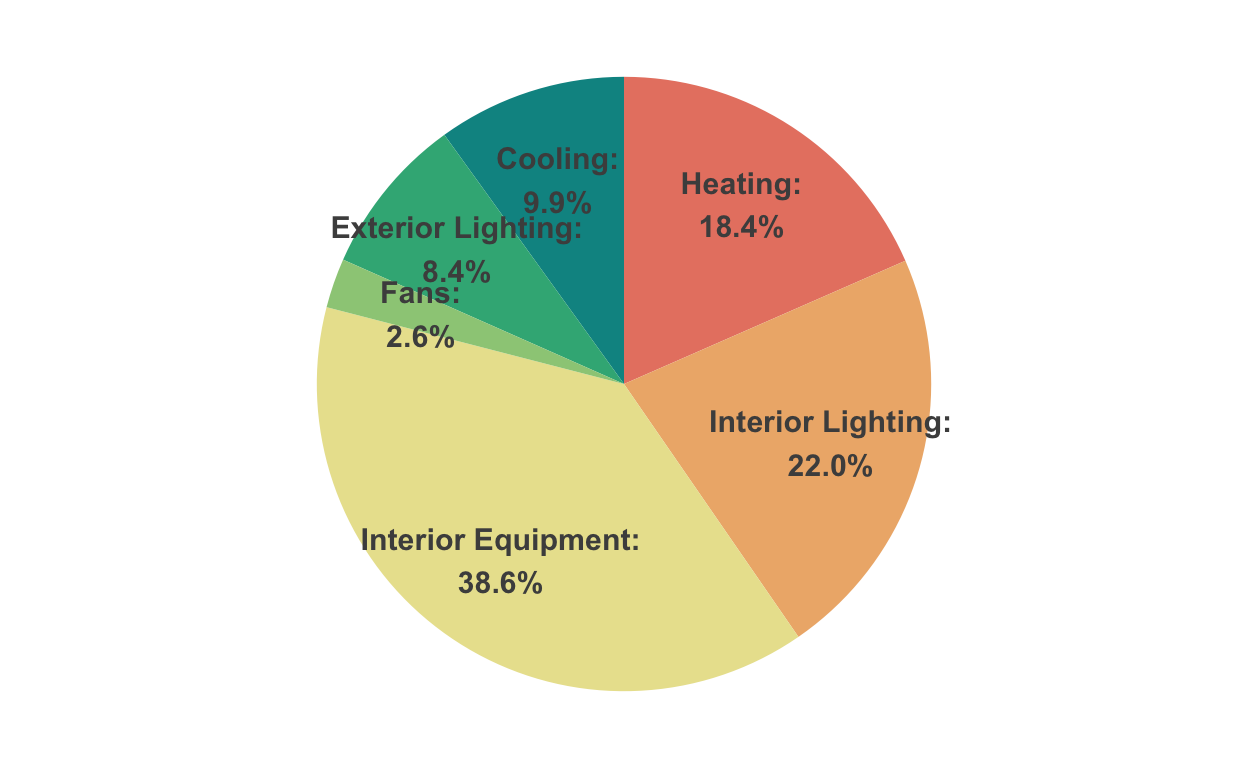
\includegraphics[width=1\linewidth]{figuresplot-1} 

}

\caption{A scatter plot}\label{fig:plot}
\end{figure}

Table \ref{tab:table} gives a result table.

\begin{table}[htbp]

\caption{\label{tab:table}A result table}
\centering
\begin{tabular}[t]{lrrrrrrrrrrr}
\toprule
  & mpg & cyl & disp & hp & drat & wt & qsec & vs & am & gear & carb\\
\midrule
Mazda RX4 & 21.0 & 6 & 160 & 110 & 3.90 & 2.620 & 16.46 & 0 & 1 & 4 & 4\\
Mazda RX4 Wag & 21.0 & 6 & 160 & 110 & 3.90 & 2.875 & 17.02 & 0 & 1 & 4 & 4\\
Datsun 710 & 22.8 & 4 & 108 & 93 & 3.85 & 2.320 & 18.61 & 1 & 1 & 4 & 1\\
Hornet 4 Drive & 21.4 & 6 & 258 & 110 & 3.08 & 3.215 & 19.44 & 1 & 0 & 3 & 1\\
Hornet Sportabout & 18.7 & 8 & 360 & 175 & 3.15 & 3.440 & 17.02 & 0 & 0 & 3 & 2\\
Valiant & 18.1 & 6 & 225 & 105 & 2.76 & 3.460 & 20.22 & 1 & 0 & 3 & 1\\
\bottomrule
\end{tabular}
\end{table}

\hypertarget{discussion}{%
\section{Discussion}\label{discussion}}

\hypertarget{conclusion}{%
\section{Conclusion}\label{conclusion}}

\hypertarget{data-availability}{%
\section*{Data availability}\label{data-availability}}
\addcontentsline{toc}{section}{Data availability}

The research compendium for this article can be found at
\url{https://github.com/YouName/RepoName}, hosted at GitHub.

\hypertarget{credit-authorship-contribution-statement}{%
\section*{CRediT authorship contribution statement}\label{credit-authorship-contribution-statement}}
\addcontentsline{toc}{section}{CRediT authorship contribution statement}

\hypertarget{acknowledgements}{%
\section*{Acknowledgements}\label{acknowledgements}}
\addcontentsline{toc}{section}{Acknowledgements}

This research was supported by \ldots{}

\renewcommand\refname{References}
\bibliography{references.bib}


\end{document}

